\documentclass[aspectratio=169, xcolor=dvipsnames]{beamer}

% --- Theme Setup ---
\usetheme{Madrid}
\usecolortheme{default}

% --- Packages ---
\usepackage{graphicx}
\usepackage{xcolor}
\usepackage{booktabs}
\usepackage{hyperref}
\usepackage{adjustbox}
\usepackage{amssymb}
\usepackage{longtable}
\usepackage{caption}

% --- Title Information ---
\title{Module 02}
\subtitle{Why DBMS?}
\author{Milav Dabgar}
\institute{www.milav.in}
\date{\today}

\begin{document}

% Title Slide
\begin{frame}
    \titlepage
\end{frame}

\begin{frame}{Module Objectives}
    \begin{itemize}
        \item To understand the need for a DBMS from a historical perspective
    \end{itemize}
\end{frame}

\begin{frame}{Module Outline}
    \begin{itemize}
        \item Evolution of data management practices
        \item History of DBMS
    \end{itemize}
\end{frame}

\section{Evolution of Data Management}

\begin{frame}
  \vfill
  \centering
  \begin{beamercolorbox}[sep=8pt,center,shadow=true,rounded=true]{title}
    \usebeamerfont{title}Evolution of Data Management\par%
  \end{beamercolorbox}
  \vfill
\end{frame}

\begin{frame}{Data Management}
    Management of Data or Records is a basic need for human society:
    \begin{itemize}
        \item Storage
        \item Retrieval
        \item Transaction
        \item Audit
        \item Archival
    \end{itemize}
    \vspace{0.5em}
    \textbf{For:}
    \begin{itemize}
        \item Individual
        \item Small / Big Enterprise
        \item Global
    \end{itemize}
    \vspace{0.5em}
    There have been two major approaches in this practice:
    \begin{itemize}
        \item Physical
        \item Electronic
    \end{itemize}
\end{frame}

\begin{frame}{Data Management: Physical}
    Physical Data or Records management, more formally known as \textbf{Book Keeping}, has been using physical ledgers and journals for centuries.
    
    \vspace{1em}
    The most significant development happened when Henry Brown, an American inventor, patented a 'receptacle for storing and preserving papers' on November 2, 1886.
    
    \vspace{1em}
    Herman Hollerith adapted the punch cards used for weaving looms to act as the memory for a mechanical tabulating machine, in 1890.
\end{frame}

\begin{frame}{Data Management: Electronic}
    Electronic Data or Records management moves with the advances in technology especially of memory, storage, computing, and networking.
    \begin{itemize}
        \item \textbf{1950s:} Computer Programming started
        \item \textbf{1960s:} Data Management with punch card / tapes and magnetic tapes
        \item \textbf{1970s:} 
        \begin{itemize}
            \item COBOL and CODASYL approach was introduced in 1971
            \item On October 14 in 1979, Apple II platform shipped VisiCalc, marking the birth of the spreadsheet
            \item Magnetic disks became prevalent
        \end{itemize}
        \item \textbf{1980s:} RDBMS changed the face of data management
        \item \textbf{1990s:} With Internet, data management started becoming global
        \item \textbf{2000s:} e-Commerce boomed, NoSQL was introduced for unstructured data management
        \item \textbf{2010s:} Data Science started riding high
    \end{itemize}
\end{frame}

\begin{frame}{Electronic Data Management Parameters}
    Electronic Data or Records management depends on various parameters including:
    \begin{columns}[t]
        \begin{column}{0.5\textwidth}
            \begin{itemize}
                \item Durability
                \item Scalability
                \item Security
                \item Retrieval
            \end{itemize}
        \end{column}
        \begin{column}{0.5\textwidth}
            \begin{itemize}
                \item Ease of Use
                \item Consistency
                \item Efficiency
                \item Cost
                \item \dots
            \end{itemize}
        \end{column}
    \end{columns}
\end{frame}

\begin{frame}{Book Keeping}
    \textbf{Recall how shop owners used to maintain their accounts.} \\
    A book register was maintained on which the shop owner wrote the amount received from customers, the amount due for any customer, inventory details and so on.
    
    \vspace{0.5em}
    \textbf{Problems with such an approach of book-keeping:}
    \begin{itemize}
        \item \textbf{Durability:} Physical damage to these registers is a possibility due to rodents, humidity, wear and tear
        \item \textbf{Scalability:} Very difficult to maintain for many years, some shops have numerous registers spanning over years
        \item \textbf{Security:} Susceptible to tampering by outsiders
        \item \textbf{Retrieval:} Time consuming process to search for a previous entry
        \item \textbf{Consistency:} Prone to human errors
    \end{itemize}
    Not only small shops but large organizations also used to maintain their transaction details in book registers.
\end{frame}

\begin{frame}{Spreadsheet Files - A better solution}
    \textbf{Spreadsheet Softwares like Google Sheets:} Due to the disadvantages of maintaining ledger registers, organizations dealing with huge amount of data shifted to using spreadsheet softwares for maintaining their records in files.
    \begin{itemize}
        \item \textbf{Durability:} These are computer applications and hence data is less prone to physical damage.
        \item \textbf{Scalability:} Easier to search, insert and modify records as compared to book ledgers
        \item \textbf{Security:} Can be password-protected
        \item \textbf{Ease of Use:} Computer applications are used to search and manipulate records in the spreadsheets leading to reduction in manpower needed to perform routine computations
        \item \textbf{Consistency:} Not guaranteed but spreadsheets are less prone to mistakes than registers.
    \end{itemize}
    \vspace{0.5em}
    \textit{Mostly useful for single user or small enterprise applications.}
\end{frame}

\begin{frame}{Why leave filesystems?}
    \textbf{Lack of efficiency in meeting growing needs}
    \begin{itemize}
        \item With rapid scale up of data, there has been considerable increase in the time required to perform most operations.
        \item A typical spreadsheet file may have an upper limit on the number of rows.
        \item Ensuring consistency of data is a big challenge.
        \item No means to check violations of constraints in the face of concurrent processing.
        \item Unable to give different permissions to different people in a centralized manner.
        \item A system crash could be catastrophic.
    \end{itemize}
    
    \vspace{0.5em}
    The above limitations of filesystems paved the way for a comprehensive platform dedicated to management of data -- the \textbf{Database Management Systems}.
\end{frame}

\section{History of DBMS}

\begin{frame}
  \vfill
  \centering
  \begin{beamercolorbox}[sep=8pt,center,shadow=true,rounded=true]{title}
    \usebeamerfont{title}History of DBMS\par%
  \end{beamercolorbox}
  \vfill
\end{frame}

\begin{frame}{History of Database Systems}
    \begin{itemize}
        \item \textbf{1950s and early 1960s:}
        \begin{itemize}
            \item Data processing using magnetic tapes for storage
            \begin{itemize}
                \item[$\triangleright$] Tapes provided only sequential access
            \end{itemize}
            \item Punched cards for input
        \end{itemize}
        \item \textbf{Late 1960s and 1970s:}
        \begin{itemize}
            \item Hard disks allowed direct access to data
            \item Network and hierarchical data models in widespread use
            \item Ted Codd defines the relational data model
            \begin{itemize}
                \item[$\triangleright$] Would win the ACM Turing Award for this work
                \item[$\triangleright$] IBM Research begins System R prototype
                \item[$\triangleright$] UC Berkeley begins Ingres prototype
            \end{itemize}
            \item High-performance (for the era) transaction processing
        \end{itemize}
    \end{itemize}
\end{frame}

\begin{frame}{History (2)}
    \begin{itemize}
        \item \textbf{1980s:}
        \begin{itemize}
            \item Research relational prototypes evolve into commercial systems -- SQL becomes industrial standard
            \item Parallel and distributed database systems
            \item Object-oriented database systems
        \end{itemize}
        \item \textbf{1990s:}
        \begin{itemize}
            \item Large decision support and data-mining applications
            \item Large multi-terabyte data warehouses
            \item Emergence of Web commerce
        \end{itemize}
        \item \textbf{Early 2000s:}
        \begin{itemize}
            \item XML and XQuery standards
            \item Automated database administration
        \end{itemize}
        \item \textbf{Later 2000s:}
        \begin{itemize}
            \item Giant data storage systems -- Google BigTable, Yahoo PNuts, Amazon, $\ldots$
        \end{itemize}
    \end{itemize}
\end{frame}

\begin{frame}{History (3): Evolution of Data Models}
    \vspace{1em}
    \begin{center}
        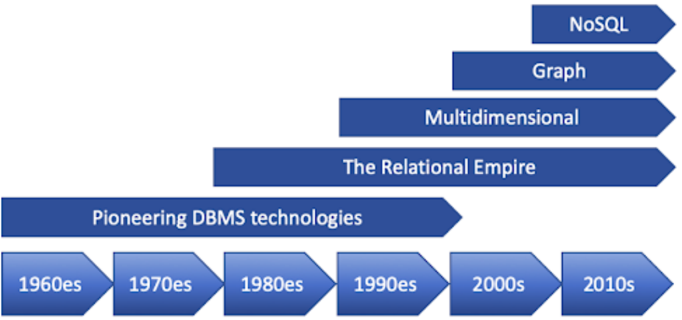
\includegraphics[height=0.7\textheight, width=0.9\textwidth, keepaspectratio]{../Lecture 1.2 - Why DBMS1_artifacts/image_000017_594d52a441b99cbcf1fe4b2919003c5fbbf44776368152ada2a471b08f0b59d5.png}
    \end{center}
\end{frame}

\begin{frame}{History (4): Evolution of DB Technology}
    \vspace{1em}
    \begin{center}
        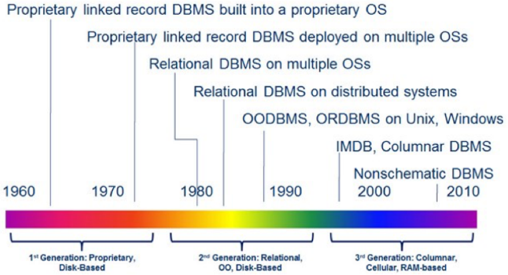
\includegraphics[height=0.7\textheight, width=0.9\textwidth, keepaspectratio]{../Lecture 1.2 - Why DBMS1_artifacts/image_000019_2b37458835a6e3db5107cdb3ae26722e3bcc3f3ffa3402aa54bd01494e29ba6e.png}
    \end{center}
\end{frame}

\begin{frame}{History (5): Evolution of DB Architecture}
    \vspace{1em}
    \begin{center}
        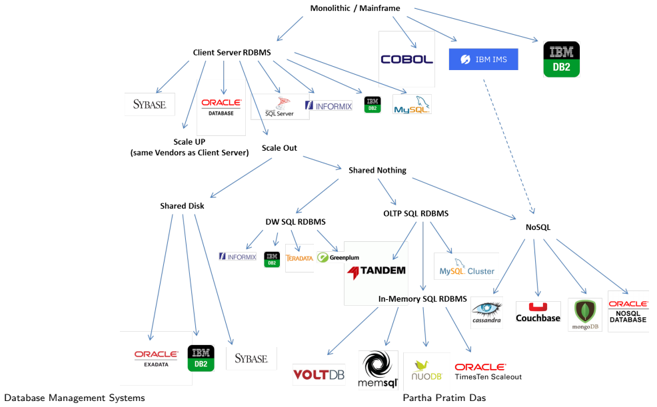
\includegraphics[height=0.7\textheight, width=0.9\textwidth, keepaspectratio]{../Lecture 1.2 - Why DBMS1_artifacts/image_000021_1de93ab87f836759d36585515f35e921eae55d607db85b06f7e9d2a0faf75074.png}
    \end{center}
\end{frame}

\begin{frame}{Module Summary}
    \begin{itemize}
        \item Walk through of evolution of Data and Records Management
        \item History of DBMS
    \end{itemize}
    
    \vspace{2em}
    \begin{center}
    \small \textit{Slides used in this presentation are borrowed from \url{http://db-book.com/} with kind permission of the authors.} \\
    \small \textit{Edited and new slides are marked with 'PPD'.}
    \end{center}
\end{frame}

\end{document}
